In this section, we evaluate the performance of our simulation tool.
We show that the inclusion of multiple synchronization protocols does not decrease our performance to the point where it is unusable.
To this end, we compare to adevs, one of the most efficient simulation kernels at this time~\cite{DEVSSurvey}.
A comparison is made for both the CPU and memory usage of both sequential simulation and parallel simulation.

We start of with a comparison of sequential simulation, to show how adevs and dxex relate in this simple case.
We not only show that our approach does not influence performance negatively, but also that our main simulation algorithm, similar to the one of PythonPDEVS, is significantly faster than the one found in adevs.
Similar differences, compared to adevs, can also be seen in the parallel simulation benchmarks.
In the parallel simulation benchmarks, the benefit of our different synchronization protocols is also indicated.

For all benchmarks, results were all well within 1\% deviation of the average, such that only the average is used in the remainder of this section.
The same compilation flags were used for both adevs and dxex benchmarks (``\texttt{-O3}'').
To guarantee comparable results, no IO was performed during the benchmarking phase.
Simulation traces were used to verify that both adevs and dxex models have exactly the same behaviour.
All benchmarks were performed using Linux, but our simulation tool works equally well on Windows and Mac.

\subsection{Benchmarks}
We use a selection of benchmarks, based on those found in the literature.
Three different types of benchmark are defined, each for a different purpose:
\begin{enumerate}
    \item \textit{Queue} model, based on the HI model of DEVStone~\cite{DEVStone}, creates a chain of atomic models, which are hierarchically nested in each other.
          A single generator will push events into the queue, which get processed by the processors after a fixed or random delay.
          It takes two parameters: width and depth, which determine the widht and depth of the hierarchy.
          This benchmark shows how the complexity of the simulation kernel behaves with an increasing amount of atomic models, and an increasingly deep hierarchy.
          If the processing delay is fixed for all processors, further insight is provided in the collision handling performance of the simulation kernel.
          An example for width 2 and depth 3 is shown in Figure~\ref{fig:queue_model}.

    \item \textit{PHOLD} model, presented by~\cite{PHOLD}.
          It creates a set of $n$ atomic models, and each model has exactly $n-1$ output ports: one for every other atomic model.
          Couplings are made such that each atomic model is directly connected to each other atomic model, such that every atomic model can directly send an event to every other atomic model.
          After a random delay, atomic models will send out an event to a randomly selected output port.
          Output port selection happens in two phases: first it is decided whether the event should be sent to an atomic model inside or outside of this coupled model.
          Afterwards, a uniform selection is made between the possible ports.
          It takes one parameter: the percentage of remote events, which influences the fraction of messages routed to other coupled models.
          This benchmark shows how the simulation kernel behaves in the presence of many local or remote events.
          An example for four models, split over two nodes, is shown in Figure~\ref{fig:PHOLD_model}.

    \item \textit{HighInterconnect} model, a merge of the HI model of DEVStone~\cite{DEVStone} and PHOLD~\cite{PHOLD}.
          It creates a structure similar to the one from PHOLD, but instead of $n-1$ output ports, every atomic model has only a single output port.
          All models are still connected to each other, but through the use of broadcasting: every model will receive a generated event.
          It takes one parameter: the number of models.
          This benchmark investigates the complexity of the routing algorithm.
          An example for four models is shown in Figure~\ref{fig:interconnect_model}.
\end{enumerate}

We opted to deviate from the DEVStone benchmark, as DEVStone tends towards unrealistic models since all internal and external transitions occur simultaneously.
In our benchmark models, there is always the option for simultaneous transition functions (\textit{fixed time advance}), or scattered transition functions (\textit{random time advance}).
Furthermore, they defined the use of an artificial load function, which easily skews the result, making the actual simulation algorithm barely comparable.

\begin{figure}
    \center
    %TODO
    %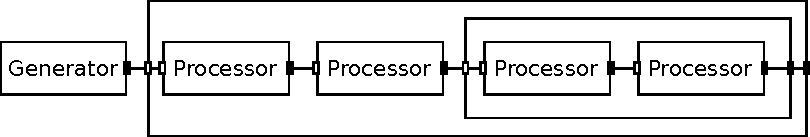
\includegraphics[width=\columnwidth]{fig/queue_model.eps}
    \caption{Queue model for depth 3 and width 2.}
    \label{fig:queue_model}

    %TODO
    %\includegraphics[width=\columnwidth]{fig/interconnect_model.eps}
    \caption{HighInterconnect model for four models.}
    \label{fig:interconnect_model}

    %TODO
    %\includegraphics[width=\columnwidth]{fig/PHOLD_model.eps}
    \caption{PHOLD model for four models, split over two nodes. In parallel simulation, each coupled model is simulated at a different node.}
    \label{fig:PHOLD_model}
\end{figure}

\subsection{Sequential Simulation Execution Time}
Despite our core contribution being mainly in the parallel simulation, we still value a comprehensive comparison of sequential simulation results.
First, and foremost, as parallel simulation results are tightly linked to the sequential simulation results: parallel simulation merely adds a synchronization layer over different, essentially sequential, simulation kernels.
Second, since parallel simulation results are validated through the use of adevs.
To provide a more comprehensive comparison to adevs in the parallel simulation benchmarks, sequential simulation results need to be compared.
Only the Queue and HighInterconnect models are relevant for sequential simulation.

\subsubsection{Queue}
In the Queue model, we increase both the width and depth simultaneously, causing a quadratic growth in the number of atomic models.
As can be seen in Figure~\ref{fig:Queue_benchmark}, dxex considerably outperforms adevs.
Through careful analysis of profiling results, we determined that adevs spends much time in handling simulation messages, whereas this is mostly avoided due to the differently designed simulation algorithm of dxex.
Both simulation tools have quadratically increasing execution times, though dxex is much faster thanks to its more efficient simulation control algorithms.

\begin{figure}
	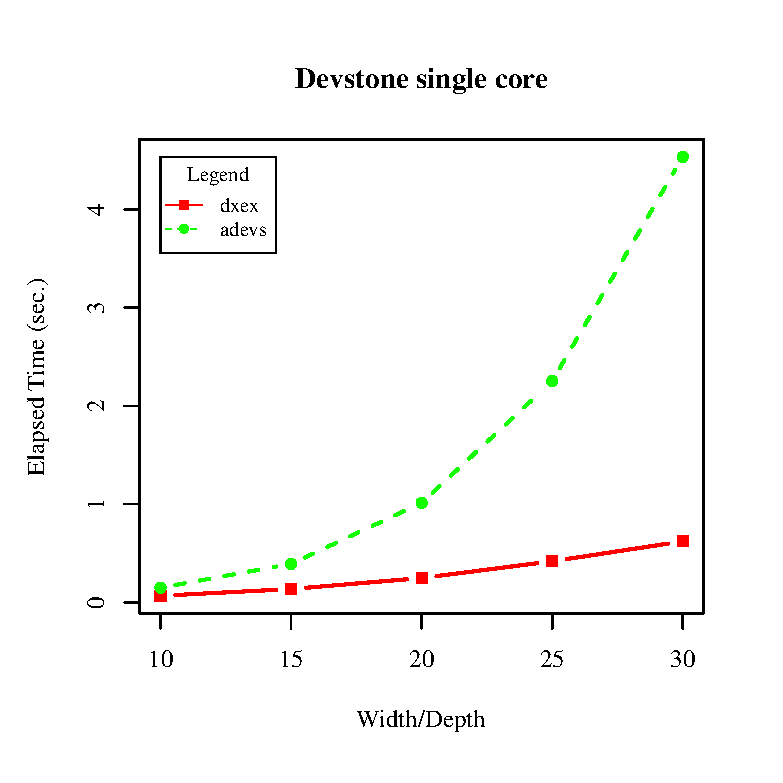
\includegraphics[width=\columnwidth]{fig/fig1.eps}
	\caption{Queue benchmark results for sequential simulation.}
	\label{fig:Queue_benchmark}
\end{figure}

\subsubsection{HighInterconnect}
In the HighInterconnect model, we increase the number of atomic models, thus quadratically increasing the number of couplings.
As can be seen in Figure~\ref{fig:Interconnect_benchmark}, adevs now outperforms dxex by a fair margin.
Analysis showed that this slowdown is caused by the high amount of exchanged events.
Event creation is found to be much slower in dxex than it is in adevs, even despite the use of memory pools in dxex.

%TODO only include sequential results?
\begin{figure}
	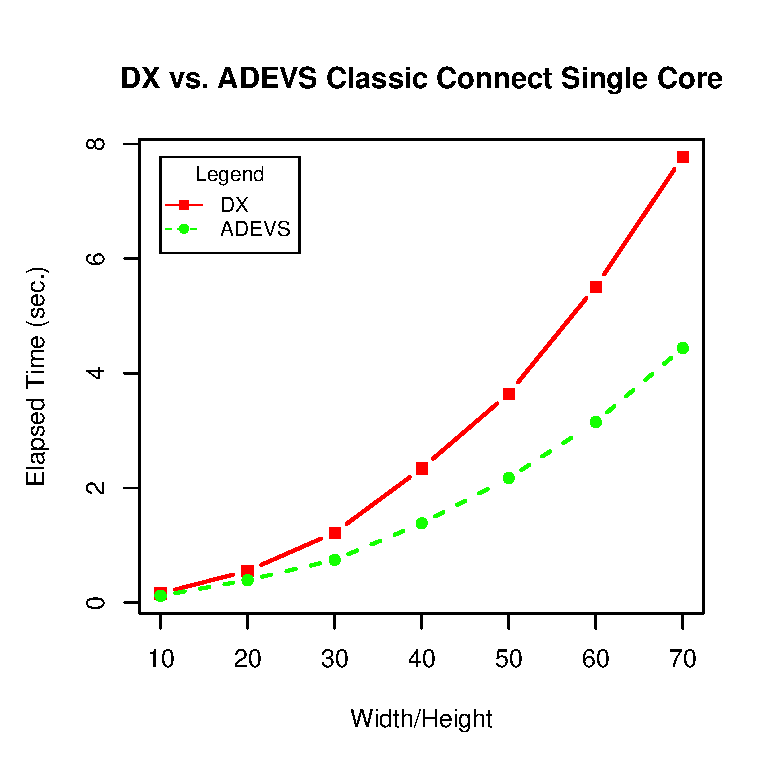
\includegraphics[width=\columnwidth]{fig/fig3.eps}
	\caption{Interconnect benchmark results for sequential simulation.}
	\label{fig:Interconnect_benchmark}
\end{figure}

\subsection{Parallel Simulation Execution Time}
We now perform an analysis of parallel simulation execution times of our previously defined benchmarks.
For dxex, we mention results for both conservative and optimistic synchronization.
Since adevs supports only conservative synchronization, we don't mention optimistic synchronization results there.
All experiments were performed using four simulation nodes, and executed on a quad-core machine.

We highlight two main results:
(1) dxex conservative synchronization is competitive with adevs;
(2) dxex optimistic synchronization is sometimes more efficient than conservative synchronization.
This shows that our contribution, offering both conservative and optimistic synchronization, is indeed beneficial for a general-purpose simulation tools.

\subsubsection{Queue}
In the Queue model, we allocate the chain of models such that each node is responsible for a series of connected models.
This minimizes the number of inter-node messages.
As the model is a queue, however, the last models will only activate much later on in the simulation.
Since these are allocated to seperate nodes, some nodes will remain idle until simulation has progressed sufficiently far.

Similar to the sequential benchmarks, Figure~\ref{fig:queue_benchmark_parallel} shows that dxex again outperforms adevs, using both optimistic and conservative synchronization.
%TODO wait for raw results to make conclusions
Behaviour is exactly the same as in sequential simulation, but some speedup is achieved.
In this case, conservative synchronization seems to be better than optimistic synchronization, at the cost of providing the lookahead.

\begin{figure}
	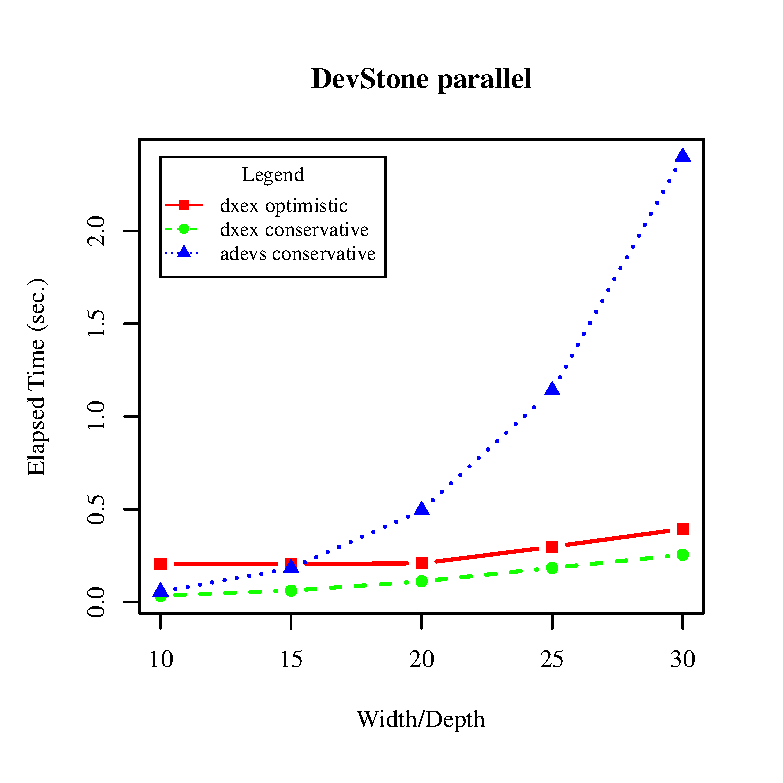
\includegraphics[width=\columnwidth]{fig/fig2.eps}
	\caption{Queue benchmark results for parallel simulation using 4 cores.}
	\label{fig:queue_benchmark_parallel}
\end{figure}

\subsubsection{PHold}
In the Phold model, we first investigate the influence of the fraction of remote events.
%TODO wait for results
%The dynamic dependency graph is a very sparse version of the static dependency graph, penalizing the conservative case. The lookahead is $\epsilon$, so the conservative case spends most of its time crawling in steps of $\epsilon$. Since the dependency graph between kernels is a complete graph, this is not a simulation that scales in our implementation. For $N$ kernels, each kernel has to query the null-time of $N-1$ kernels, resulting in O($N^2$) polling behaviour. In a non-cyclic simulation with a non-trivial lookahead (like in, e.g., Devstone), that choice does pay off (see Figure~\ref{fig:DevstoneParallel}). Adevs's lesser performance is due in part to their lookahead management, which after profiling shows to spend a non-trivial amount of time in exception handling code.\\
%The optimistic case suffers little from the above problems; due to the high interconnectivity, however, a cascading revert is still possible. With the percentage of remotes equal to $100$, Phold reflects interconnect in behaviour, which is why the $R$ value is not dimensioned here. A revert is very expensive in PHold due to our usage of C++11's random nr generators. The cost of a revert is dominated by the recalculation of destination models, not in allocating/deallocating states/messages. Once a revert happens the drift between kernels increases fast, increasing the likelihood of more reverts. Despite all this, optimistic can for low $R$ values quickly exploit the uncertainty that slows down conservative in this benchmark.

Secondly, we verify that our contribution fulfills our projected use case: a single model that can be tweaked to favor either conservative or optimistic synchronization.
We slightly modified the Phold benchmark, to include high-priority events.
Contrary to normal events, which offer a sufficiently large lookahead, high-priority events happen almost instantaneous, thus restricting lookahead to a very small value.
Even though the normal events will occur most oftenly, a conservative implementation should always block since these high-priority events can always occur.
An optimistic implementation, however, will simply go forward in simulation time and roll back the few times that these high-priority events happen.
This situation closely mimics the case made in the comparison between both synchronization algorithms by~\cite{FujimotoBook}.

Figure~\ref{fig:phold_priority} shows how simulation performance is influenced by the fraction of high-priority events.
If barely any high-priority events occur, conservative synchronization is penalized due to its excessive blocking, which often turned out to be unnecessary.
Should many high-priority events occur, however, optimistic synchronization is penalized due to its mindless progression of simulation, which frequently needed to be reverted.

\begin{figure}
    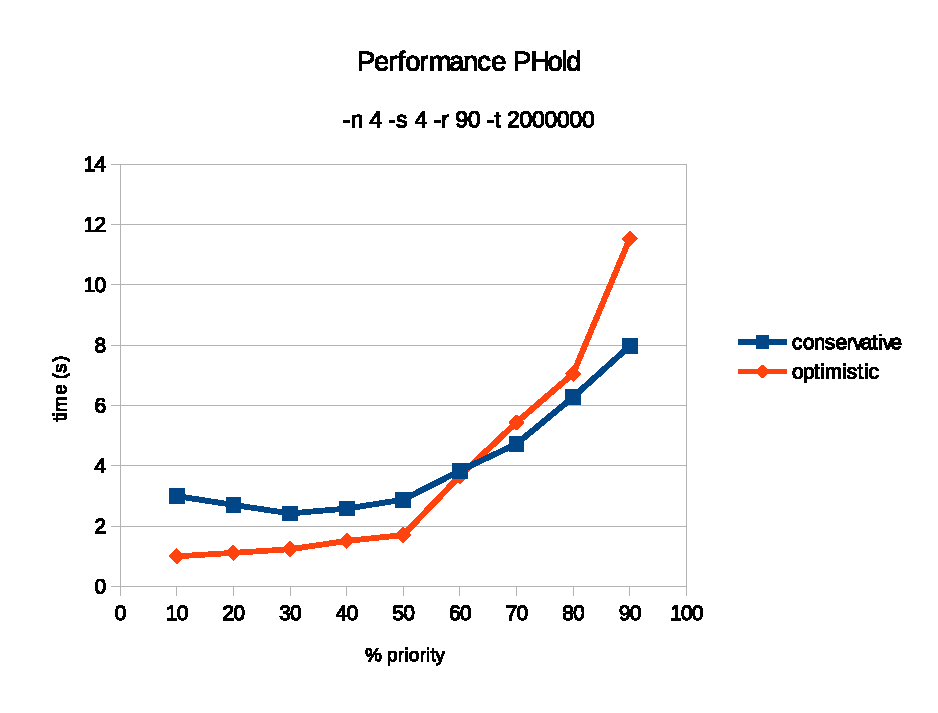
\includegraphics[width=\columnwidth]{fig/phold_voorlopig.eps}
    \caption{Phold benchmark results with high-priority events.}
    \label{fig:phold_priority}
\end{figure}

\subsubsection{Interconnect}
In Interconnect, the set of atomic models form a complete graph (w.r.t. connections); each model broadcasts messages to the entire set.\\
Allocation cannot avoid cycles and the resulting dependency graph between kernels remains a complete graph. The runtime dependency graph is almost immediately identical to the static graph.\\
The conservative case still shows the same issues as in PHold, with the key difference , for a fixed time advance, the lookahead is equal to the timespan between transitions. The scaling issue is identical as with PHold.\\
In this benchmark, the optimistic case runs very quickly out of memory. With $c$ kernels and $N$ atomic models, a single revert undoing $k$ transitions will lead to $(N-1)\times k$ messages that need to be recreated, plus $(N-1) \frac{c-1}{c} \times k$ anti-messages that need to be sent.

\subsubsection{Priority network model}
%TODO show a single plot which varies a parameter that changes the ideal synchronization protocol
The priority benchmark is composed of a single server generating a stream of $0\leq m \leq n$ messages at fixed time intervals, interleaved with a probability $p$ for a priority message to $n$ receivers (see Figure~\ref{fig:NetworkModel}).\\ This defaults the lookahead for the receivers to $\epsilon$, but this time there is no scaling effect, nor are there cycles in the dependency graph. This model therefore highlights the basic strengths/weaknesses of both synchronization protocols. Receiving models are allocated on another kernel than the server and have an internal transition so that they will not wait for the incoming messages.
\begin{center}
\begin{figure}
\input pqueue.tex
\caption{The priority network model}
\label{fig:NetworkModel}
\end{figure}
\end{center}
A key difference here with the other benchmarks is that a state (in the Receiver instances) is very cheap to copy/create. The kernel holding the server will never revert since it is a source in the dependency graph. The optimistic case will therefore not suffer the same performance hit in recreating the states as it does in PHold. The overhead in the optimistic case is entirely due to the factor $m$, which will quickly dominate in increasing buffers of received messages.
\begin{figure}
	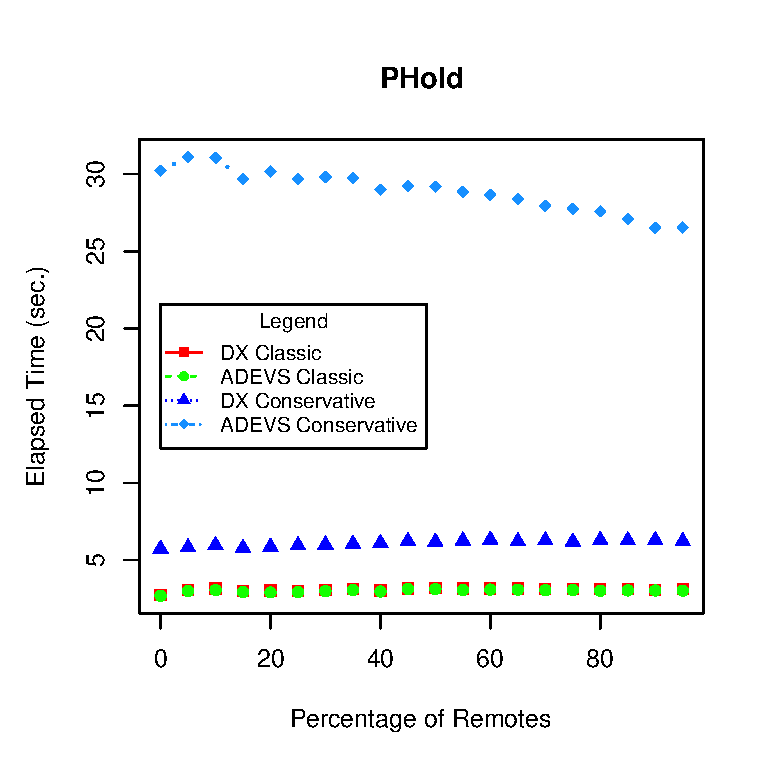
\includegraphics[width=.5\textwidth]{fig/fig5.eps}
	\label{fig:Priority}
	\caption{Priority}
\end{figure}
Interestingly, the parameter $p$ does not clearly favour either synchronization protocol (see Figure~\ref{fig:Priority}). While this removes any possibility for a lookahead, the conservative case can quickly bridge the timespan between fixed messages since there is no cyclic dependency. Lightweight states prevent performance loss due to reverts in the optimistic case; only the overhead in event handling in the optimistic case eventually becomes the deciding factor.

%TODO (keep explaining as much as space permits, as this is the evaluation of the core contribution)
\subsection{Memory Usage}
%TODO compare memory usage with adevs for some benchmarks
\subsubsection{Platform and tools}
Both dxex and adevs use tcmalloc as memory allocator. Additionally, dxex uses memory pools to further reduce the frequency of expensive system calls (malloc/free/sbrk/mmap/...). Tcmalloc will only gradually release memory back to the OS, whereas our pools will not do so at all. If memory has been allocated once, it is from a performance point of view better to keep that memory in the pool. This is one reason why memory utilization is best measured by peak allocation. Profiling is done using Valgrind's massif tool~\cite{Nethercote:2007:VFH:1273442.1250746}.
The platform used for memory profiling has an i5-3317U Intel CPU and 8GiB RAM with a page size of 4,096KiB, running Fedora 22 (kernel 4.2.6).
\subsubsection{Measure}
Adevs passes messages by value, dxex passes a pointer. The runtime effects of this choice have already been demonstrated in the Interconnect benchmark, so, in this section, we measure memory usage in number of allocated pages combining text, stack and heap memory for the program profiled. For the OS and/or user, this is the actual memory footprint of the application. It is important to note that, especially in the optimistic case, not all this memory is always in use by the kernels. During simulation, the pools will generally not return deallocated memory to the OS, but keep it for later reuse.
\subsubsection{Results}
\paragraph*{Devstone}
\begin{table}[htb]
	\centering
	\begin{tabular}{| l | l | l | l | l |}
		\hline
		adevs & adevs con &dxex &dxex con&dxex opt\\ \hline
		44 & 70 & 42 & 75 & 363  \\ \hline
	\end{tabular}
	\caption{Devstone 40x40 t5e5, unit MiB, 4 kernels (if parallel)}
\end{table}
Since, in the conservative case, messages are passed by pa ointer, a GVT/LBTS implementation is required to organise the garbage collection. This inevitable delay explains the higher memory usage compared to adevs.\\
%TODO next sentence needs rewriting --done?
Optimistic's TimeWarp requires state/event saving, and its GVT algorithm is more complex (with a resulting higher latency) than the LBTS calculation in the conservative case. 
Moreover, the differences in LP virtual times are far larger compared to conservative time synchronization. All these factors explain the heavier memory usage. Devstone (flattened) is allocated in a chain. Leafs in the dependency graph will therefore do a lot of unnecessary simulation before having a revert, leading to an increased memory pressure. Unlike conservative and sequential execution, memory usage in the optimistic case varies greatly depending on scheduling of kernel threads and drifting between kernels. 
\paragraph*{PHold}
\begin{table}[htb]
	\centering
	\begin{tabular}{| l | l | l | l | l |}
		\hline
		adevs & adevs con &dxex &dxex con &dxex opt\\ \hline
		40 & x & 37 & 61 & 682  \\ \hline
	\end{tabular}
	\caption{Phold n 4 s 16 t1e6 r 10, unit MiB, 4 kernels (if parallel)}
\end{table}
With only 10\% of all messages being inter-kernel, we expect conservative to have memory consumption near that of the single threaded implementation, since intra-kernel messages are reclaimable after each round. The counterintuitive high memory usage can be explained by conservative's stalled round behaviour which occurs whenever a kernel cannot advance (eit $==$ time). In such a round messages are sent out but the kernel does not execute any transitions until it has received all input from all influencing kernels. \\
With lookahead $\epsilon$ this then leads to a high frequency of polling on shared null-times, which are used to determine lbts and thus garbage collection.
The lbts calculation will not wait until a new value is found, since this can create unwanted contention with the simulation. The resulting longer time intervals within which no new lbts is found delay memory deallocation.
Adevs' conservative fails to complete the benchmark under valgrind even with a significantly reduced load.
Optimistic exhibits the expected high memory usage.
\paragraph*{Interconnect}
In section 4.2 the parallel performance of this benchmark is further explained. Interconnect highlights dxex's lower performance due to message allocation overhead. 
\begin{table}
	\centering
	\begin{tabular}{| l | l | l | l | l |}
		\hline
		adevs & adevs con &dxex &dxex con & dxex opt\\ \hline
		39 & 39 & 35 & 43 & 259 \\ \hline
	\end{tabular}
	\caption{Interconnect w 20 t5e5, unit MiB, 2 kernels (if parallel)}
\end{table}
		
\paragraph*{Priority Network}
The priority network model is detailed in section 4.1.\\
The high memory usage of the conservative case is largely due to the garbage collection implementation. Kernel 0 is the initiator of the LBTS calculation but since it holds only models independent of any other (server), it will finish simulation very fast leaving the other kernel bereft of an updated LBTS. The kernel holding the server will after simulation wait on the receiving kernel until it can prove all sent messages can be deallocated.
\begin{table}
	\centering
	\begin{tabular}{| l | l | l |}
		\hline
		dxex &dxex con &dxex opt\\ \hline
		35 & 450 & 651\\ \hline
	\end{tabular}
	\caption{Priority model n 128, m 16, p 10,  t2e8, unit MiB, 2 kernels}
\end{table}
